\section{Resultados para o controlador por \textit{state feedback}}

\subsection{Projeto dos circuitos}

Tendo em mente a identificação das variáveis de estado como funções do sinal de saída já demonstradas na parte de projeto, o circuito da planta pode ser reaproveitado para o projeto por realimentação de estados. Isso é possível pois o nó de saída do integrador prático é exatamente a derivada invertida de y(t). Em suma, as alterações feitas estão presentes nos ganhos e no subtrator, sendo topologias padrões retiradas da bibliografia consultada. 


\begin{figure}[H]
\begin{center}
    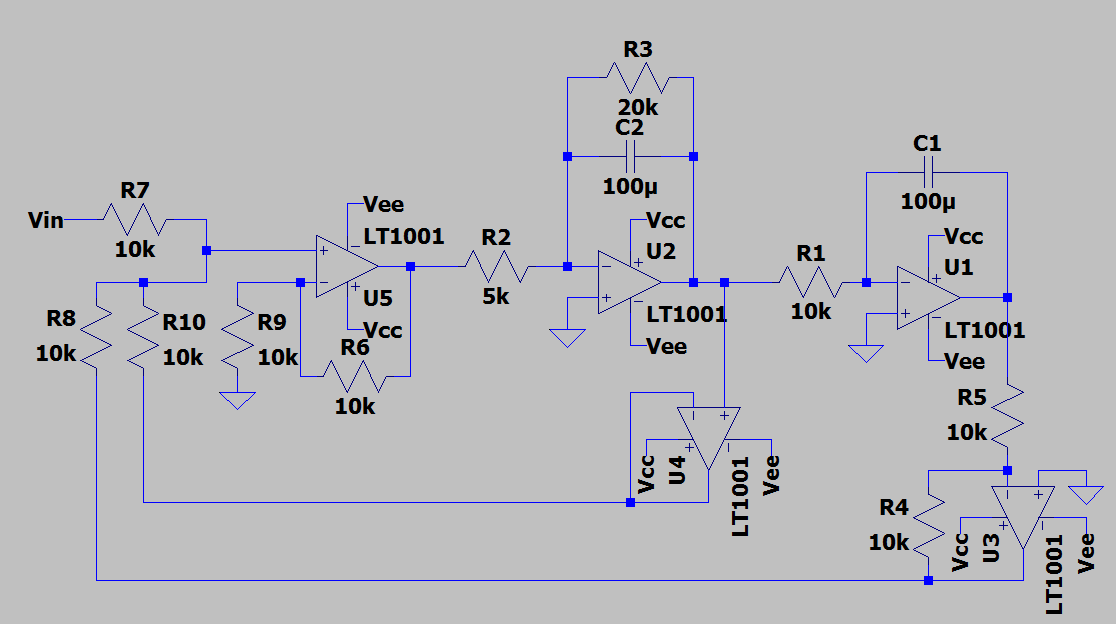
\includegraphics[width=16cm]{images/state/circuitoLT.png}  
\end{center}
\caption{Circuito proposto para realimentação de estados.}
\label{rea:1} 
\end{figure}

Com isso, a topologia do circuito está ilustrada na figura \ref{rea:1} e seu resultado montado em protoboard na figura \ref{rea:2}, obtendo, assim, um circuito bem planejado e compacto.

\subsection{Simulações no LTspice}

Analisando o circuito montado no LTspice do circuito com realimentação de estados (figura \ref{rea:1}), podemos notar um resultado bem próximo do esperado.  

\begin{figure}[H]
\begin{center}
    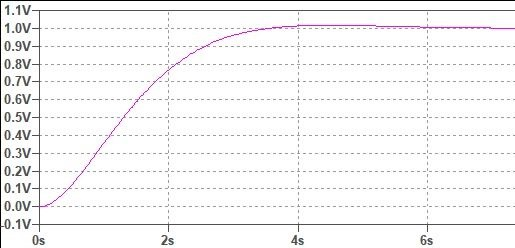
\includegraphics[width=12cm]{images/state/simulacao.jpg}  
\end{center}
\caption{Simulação do circuito de realimentação de estados no LTspice.}
\label{rea:3} 
\end{figure}

Nota-se que no tempo, para os parâmetros estipulados e o percentual de overshoot, obtemos um percentual em torno dos 5\%, além de tempo de estabilização muito bom, em torno dos 4 segundos.

\subsection{Resultados práticos}

Foi realizada a montagem do circuito projetado no protoboard(figura \ref{rea:2}) e em seguida mediu-se no osciloscópio o sinal resultante.

\begin{figure}[H]
\begin{center}
    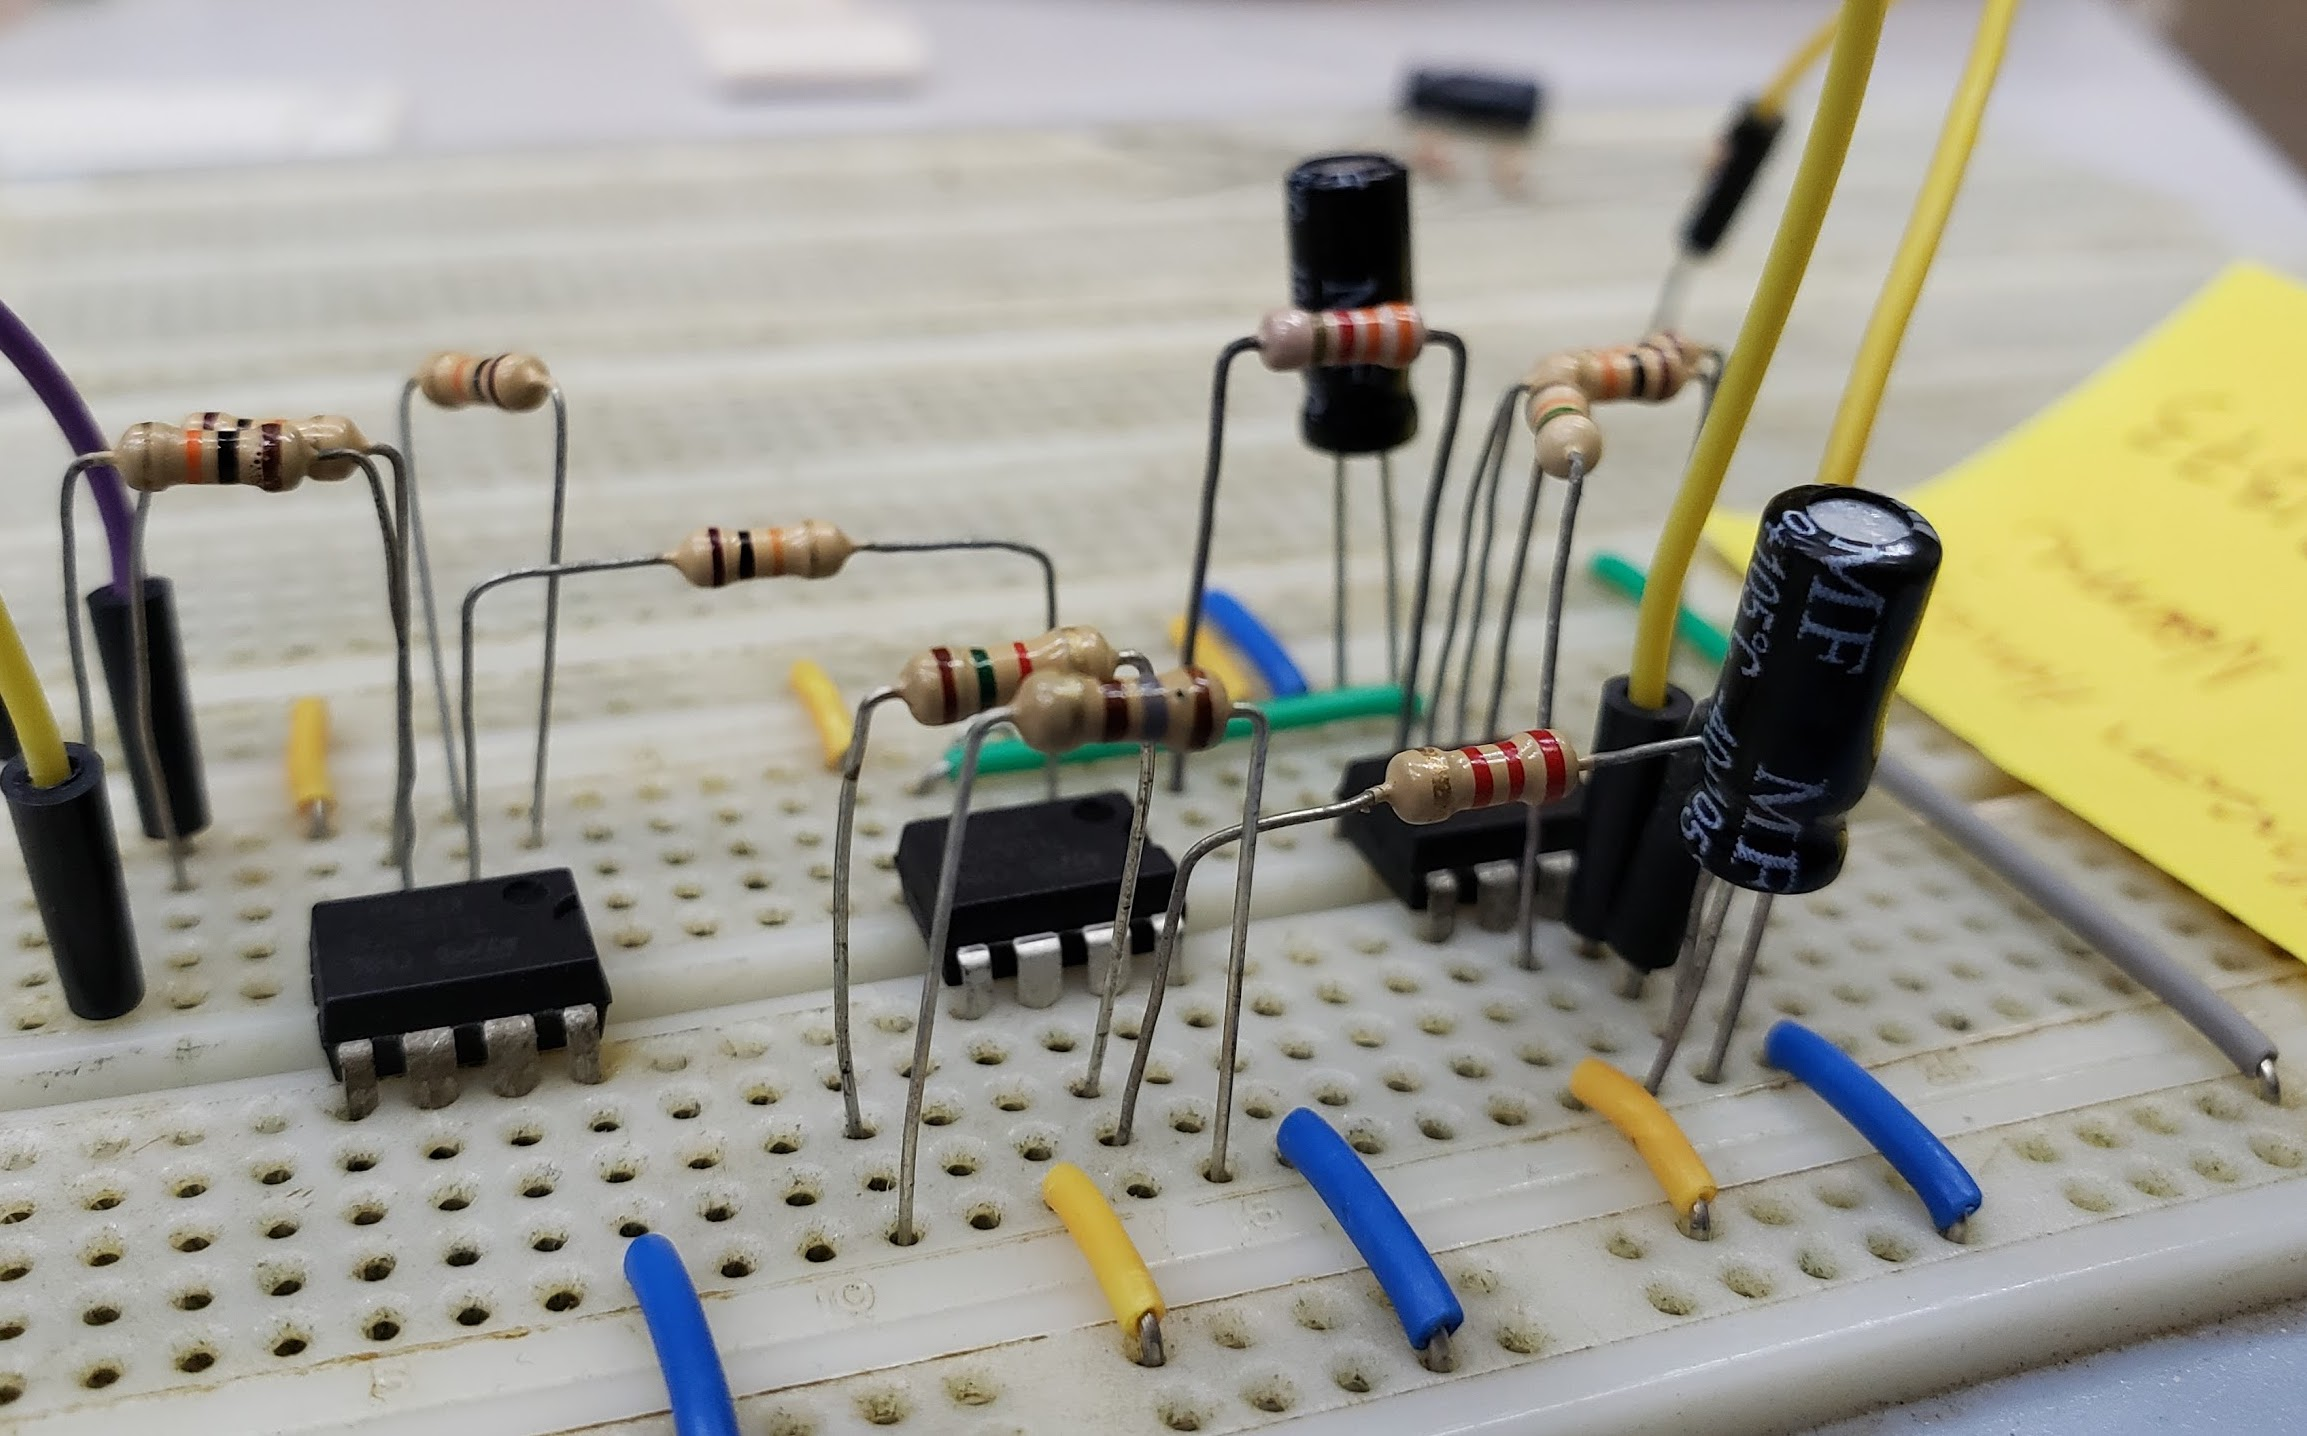
\includegraphics[width=10cm]{images/state/circ_controle.jpeg}  
\end{center}
\caption{Circuito de realimentação de estados montado em protoboard.}
\label{rea:2} 
\end{figure}

Os ganhos foram distribuídos entre o somador não inversor, de forma que as divergências causadas pela utilização de valores comerciais de resistores originou um pequeno, porém não desprezível, erro em regime permanente. 

Ademais, em relação ao tempo de estabilização, podemos observar na figura \ref{rea:4} que a saída se estabiliza em 3,44s, estando dentro do tempo esperado de 4s.

\begin{figure}[H]
\begin{center}
    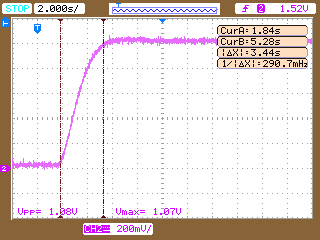
\includegraphics[width=10cm]{images/state/State1.png}  
\end{center}
\caption{Sinal resultante - Tempo de estabilização.}
\label{rea:4} 
\end{figure}

Com relação ao percentual de overshoot, conseguimos visualizar na imagem \ref{rea:5} e calcular a partir da fórmula a seguir: 

\begin{equation} \label{g:PO}
    PO\% = (Vmax-1)*100 = (1.02-1)*100 =2\%
\end{equation}

\begin{figure}[H]
\begin{center}
    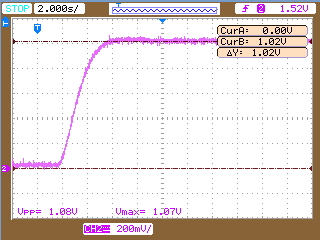
\includegraphics[width=10cm]{images/state/State0.png}  
\end{center}
\caption{Sinal resultante - percentual de overshoot.}
\label{rea:5} 
\end{figure}

\pagebreak

